\documentclass[11pt]{article}
% Shared preamble for the printable mini lessons (1.4 onward).
%   \documentclass[11pt]{article}
%   \input{../preamble}
% Build the key with:  pdflatex -jobname=<name>_KEY "\def\iskey{}\input{<name>}"
% Figures shared with the web page live in figures/Unit_X/<name>.tex and are
% pulled in with \fig{Unit_X/<name>}; the standalone package drops their own
% preamble, so their macros come from figures/preamble.tex, loaded here.
% Shared preamble for web figures.  Each figure is a standalone .tex that
% \input's this file; scripts/make-figures.sh turns it into an SVG.
\usepackage[T1]{fontenc}
\usepackage{helvet}
\renewcommand{\familydefault}{\sfdefault}
\usepackage{tikz}
\usetikzlibrary{decorations.pathreplacing}
% axis numbers in the text font, not math italic
\pgfkeys{/pgf/number format/.cd,assume math mode=true,1000 sep={}}

% dot plot: \dotplot{min}{max}{value/count,...}{axis label}
\newcommand{\dotplot}[4]{%
\begin{tikzpicture}[x=0.9cm,y=0.33cm]
  \draw[thick] (#1-0.5,0) -- (#2+0.5,0);
  \foreach \t in {#1,...,#2} {\draw (\t,0.25) -- (\t,-0.25) node[below] {\t};}
  \foreach \v/\c in {#3} {\ifnum\c>0 \foreach \k in {1,...,\c} {\fill (\v,\k*1.15) circle (0.16cm);}\fi}
  \node at ({(#1+#2)/2},-2.3) {#4};
\end{tikzpicture}}

% shape sketch histogram (12 bins): \shapehist{heights}{label}
\newcommand{\shapehist}[2]{%
  \foreach \h [count=\i from 0] in {#1} \draw[fill=gray!30] (\i,0) rectangle (\i+1,\h);
  \draw (-0.3,0) -- (12.3,0);
  \node[font=\bfseries] at (6,-2.6) {#2};}
\newcommand{\meanmark}[1]{\fill (#1,0) -- ++(-0.3,-0.75) -- ++(0.6,0) -- cycle;}
\newcommand{\medmark}[2]{\draw[very thick,dashed] (#1,0) -- (#1,#2);}

% number line with minor ticks: \nline{min}{max}{label step}{axis label}
\newcommand{\nline}[4]{%
  \draw[thick] (#1-0.5,0) -- (#2+0.5,0);
  \foreach \t in {#1,...,#2} \draw (\t,0.12) -- (\t,-0.12);
  \pgfmathtruncatemacro{\nxt}{#1+#3}
  \foreach \t in {#1,\nxt,...,#2} \draw (\t,0.2) -- (\t,-0.2) node[below] {\t};
  \node at ({(#1+#2)/2},-0.95) {#4};}
% box plot above the line: \bplot{min}{Q1}{med}{Q3}{max}
\newcommand{\bplot}[5]{%
  \draw[thick] (#1,1.0) -- (#2,1.0);
  \draw[thick] (#4,1.0) -- (#5,1.0);
  \draw[thick] (#1,0.75) -- (#1,1.25);
  \draw[thick] (#5,0.75) -- (#5,1.25);
  \draw[thick,fill=gray!20] (#2,0.55) rectangle (#4,1.45);
  \draw[very thick] (#3,0.55) -- (#3,1.45);}

% ---- added for 1.4 onward ----
% axis on y=0: \axis{min}{max}{label step}{tick step}{axis label}
\newcommand{\axis}[5]{%
  \draw[thick] (#1,0) -- (#2,0);
  \pgfmathsetmacro{\axT}{#1+#4}\foreach \t in {#1,\axT,...,#2} \draw (\t,0.1) -- (\t,-0.1);
  \pgfmathsetmacro{\axL}{#1+#3}\foreach \t in {#1,\axL,...,#2}
    \draw (\t,0.18) -- (\t,-0.18) node[below] {\pgfmathprintnumber{\t}};
  \node at ({(#1+#2)/2},-0.95) {#5};}
% box plot centred at height y: \bplotat{y}{min}{Q1}{med}{Q3}{max}
\newcommand{\bplotat}[6]{%
  \draw[thick] (#2,#1) -- (#3,#1);
  \draw[thick] (#5,#1) -- (#6,#1);
  \draw[thick] (#2,#1-0.22) -- (#2,#1+0.22);
  \draw[thick] (#6,#1-0.22) -- (#6,#1+0.22);
  \draw[thick,fill=gray!20] (#3,#1-0.42) rectangle (#5,#1+0.42);
  \draw[very thick] (#4,#1-0.42) -- (#4,#1+0.42);}
% an outlier dot: \outlier{x}{y}
\newcommand{\outlier}[2]{\fill (#1,#2) circle (2.4pt);}

\usepackage[margin=0.75in]{geometry}
\usepackage{array}
\usepackage{enumitem}
\usepackage{amsmath}
\usepackage[helvet]{sfmath}  % math in the same sans font as the text
\usepackage{standalone}
\pagestyle{empty}
\setlength{\parindent}{0pt}
\setlist[enumerate,1]{leftmargin=1.5em,itemsep=1em}
\setlist[enumerate,2]{label=(\alph*),leftmargin=2em,itemsep=2.2em}

\newif\ifkey
\ifdefined\iskey \keytrue \fi
\colorlet{keyred}{red!75!black}
\newcommand{\ans}[1]{\ifkey\leavevmode{\color{keyred}#1}\fi}
% vertical work space on the student copy, less on the key
\newcommand{\work}[1]{\ifkey\vspace{0.6em}\else\vspace{#1}\fi}
\newcommand{\fig}[1]{\input{../../figures/#1}}
% Title line: \lessontitle{Quartiles, IQR, and Box Plots}
\newcommand{\lessontitle}[1]{{\Large\bfseries #1\ifkey\ \textcolor{keyred}{KEY}\fi}\hfill Name \underline{\hspace{2in}}\par\vspace{0.6em}}
\newcommand{\partner}{\par\vspace{0.4em}Work with a partner. Compare answers when you finish each problem.\par}

% Unit quiz: two questions per mini lesson, each headed by the lesson's
% objective.  The key keeps every box the same height as the student copy,
% so key page N lines up with quiz page N.
\newcommand{\lessonhead}[1]{\par\vspace{0.6em}{\large\bfseries #1}\par\vspace{0.25em}\hrule\vspace{0.6em}}
\newcommand{\goal}[1]{\textbf{#1}\par\vspace{0.35em}}
% answer box: same height on both copies, answer printed only on the key
\newcommand{\abox}[2]{\par\begin{minipage}[t][#1][t]{\linewidth}\raggedright\vspace{0.2em}\ans{#2}\end{minipage}\par}
\newcommand{\tally}[1]{\tikz[baseline=0pt]{\foreach \i in {1,...,#1} \draw[line width=0.7pt] (\i*0.08,0) -- (\i*0.08,0.22);}}
% circled choices: \opt{A} prints plain; \optans{B} is circled in red on the key
\newcommand{\opt}[1]{\tikz[baseline=(c.base)]\node[rounded corners=0.6em,inner sep=2.5pt](c){#1};}
\newcommand{\optans}[1]{\ifkey\tikz[baseline=(c.base)]\node[rounded corners=0.6em,inner sep=2.5pt,draw=keyred,thick,text=keyred](c){#1};\else\opt{#1}\fi}
% five-number summary blanks, filled in red on the key
\newcommand{\fsblank}[1]{\underline{\makebox[0.65in]{\ans{#1}}}}
\newcommand{\fivesum}[5]{\par Min \fsblank{#1}\quad Q1 \fsblank{#2}\quad Median \fsblank{#3}\quad Q3 \fsblank{#4}\quad Max \fsblank{#5}\par}
\setlist[enumerate,2]{label=(\alph*),leftmargin=2em,itemsep=0.3em}
\setlist[enumerate,1]{leftmargin=1.5em,itemsep=1em}
\raggedright\hyphenpenalty=10000\exhyphenpenalty=10000

\begin{document}

\lessontitle{Unit 1 Quiz: Displaying One Variable}

Show your work.

% ======================================================================
\lessonhead{1.1 - Frequency Tables, Dot Plots, and Histograms}
\begin{enumerate}

\item \goal{I make and read a frequency table and a dot plot.}
16 students said how many languages they speak.
\begin{center}2,\; 1,\; 3,\; 2,\; 4,\; 2,\; 1,\; 3,\; 2,\; 3,\; 2,\; 1,\; 5,\; 2,\; 3,\; 2\end{center}
\begin{minipage}[t]{0.47\linewidth}\vspace{0pt}\raggedright
\begin{enumerate}
  \item Make a frequency table.

  \vspace{0.5em}
  \renewcommand{\arraystretch}{1.3}
  \begin{tabular}{|c|p{0.8in}|p{0.75in}|} \hline
  Languages & Tally & Frequency \\ \hline
  1 & \ans{\tally{3}} & \ans{3} \\ 2 & \ans{\tally{7}} & \ans{7} \\ 3 & \ans{\tally{4}} & \ans{4} \\ 4 & \ans{\tally{1}} & \ans{1} \\ 5 & \ans{\tally{1}} & \ans{1} \\ \hline
  \end{tabular}
\end{enumerate}
\end{minipage}\hfill
\begin{minipage}[t]{0.49\linewidth}\vspace{0pt}\raggedright
\begin{enumerate}[start=2]
  \item Make a dot plot.

  \vspace{0.5em}
  \begin{center}
  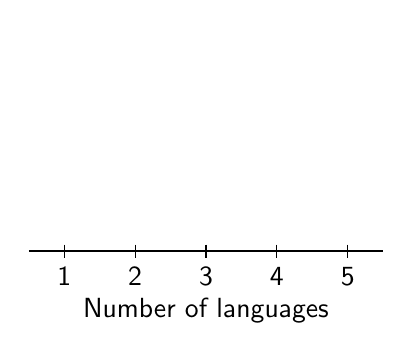
\begin{tikzpicture}[x=0.9cm,y=0.33cm]
    \draw[thick] (0.5,0) -- (5.5,0);
    \foreach \t in {1,...,5} {\draw (\t,0.25) -- (\t,-0.25) node[below] {\t};}
    \node at (3,-2.3) {Number of languages};
    \path (1,0) -- (1,8.6);
    \ifkey\foreach \v/\c in {1/3,2/7,3/4,4/1,5/1} {\foreach \k in {1,...,\c} {\fill[keyred] (\v,\k*1.15) circle (0.16cm);}}\fi
  \end{tikzpicture}
  \end{center}
\end{enumerate}
\end{minipage}

\vspace{0.6em}
\begin{enumerate}[start=3]
  \item How many students speak 3 or more languages?
  \abox{1.8em}{$4 + 1 + 1 = 6$ students}
\end{enumerate}

\item \goal{I read a histogram.}
This histogram shows the lengths of 30 songs on a playlist.

\begin{minipage}[t]{0.47\linewidth}\vspace{0pt}\raggedright
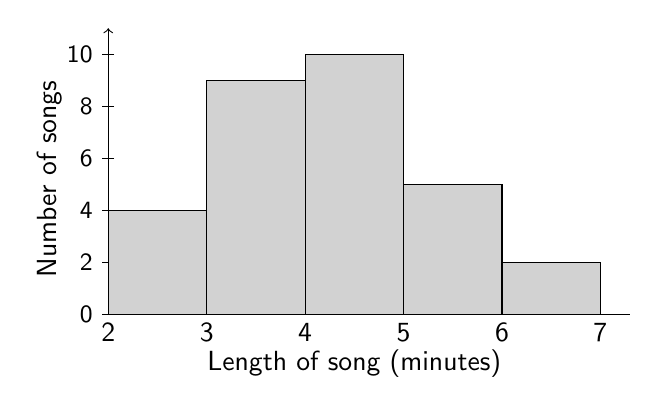
\begin{tikzpicture}[x=1.25cm,y=0.33cm]
  \draw[->] (2,0) -- (2,11); \draw (2,0) -- (7.3,0);
  \foreach \y in {0,2,...,10} \draw (2.06,\y) -- (1.94,\y) node[left,font=\small] {\y};
  \foreach \l/\h in {2/4,3/9,4/10,5/5,6/2} \draw[fill=gray!35] (\l,0) rectangle (\l+1,\h);
  \foreach \l in {2,...,7} \node[below] at (\l,0) {\l};
  \node[rotate=90] at (1.4,5.2) {Number of songs};
  \node at (4.5,-1.9) {Length of song (minutes)};
\end{tikzpicture}
\end{minipage}\hfill
\begin{minipage}[t]{0.5\linewidth}\vspace{0pt}\raggedright
\begin{enumerate}
  \item How many songs are from 3 to 4 minutes long?
  \abox{1.3em}{9 songs}
  \item How many songs are 5 minutes long or longer?
  \abox{1.3em}{$5 + 2 = 7$ songs}
  \item One song is exactly 4 minutes long. Which bar is it in?
  \abox{2.6em}{The 4 to 5 bar. A value on the line goes in the bar on the right.}
  \item Can you tell from the graph how long the longest song is? Explain.
  \abox{3.6em}{No. The graph only shows that it is from 6 to 7 minutes long. A histogram hides the exact values.}
\end{enumerate}
\end{minipage}

\end{enumerate}

% ======================================================================
\newpage
\lessonhead{1.2 - Mean, Median, and Shape}
\begin{enumerate}[resume]

\item \goal{I find the mean and the median of a data set.}
A basketball player scored these points in 6 games.
\begin{center}14,\; 9,\; 21,\; 12,\; 9,\; 19\end{center}
\begin{enumerate}
  \item Find $\Sigma x$.
  \abox{4em}{$\Sigma x = 14 + 9 + 21 + 12 + 9 + 19 = 84$}
  \item Find the mean, $\bar{x}$.
  \abox{4.5em}{$n = 6$, \quad $\bar{x} = \frac{\Sigma x}{n} = \frac{84}{6} = 14$ points}
  \item Find the median.
  \abox{4.5em}{In order: 9, 9, \fbox{12}, \fbox{14}, 19, 21. \quad Median $= (12 + 14) \div 2 = 13$ points}
\end{enumerate}

\item \goal{I tell the shape of a graph, and I choose the best measure of center.}
This histogram shows the scores of 60 students on a test.

\begin{minipage}[t]{0.47\linewidth}\vspace{0pt}\raggedright
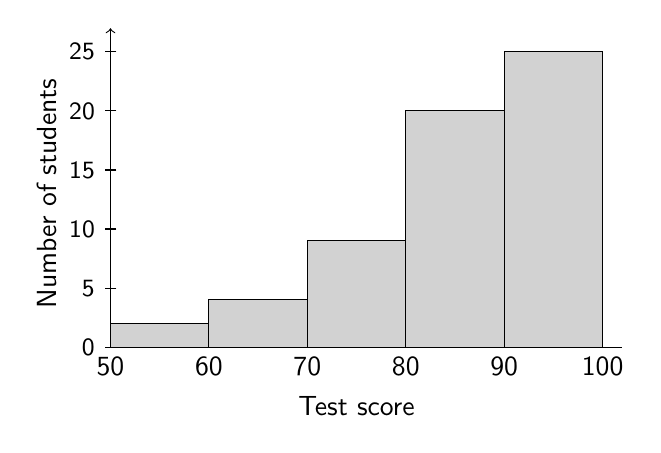
\begin{tikzpicture}[x=0.125cm,y=0.15cm]
  \draw[->] (50,0) -- (50,27); \draw (50,0) -- (102,0);
  \foreach \y in {0,5,...,25} \draw (50.6,\y) -- (49.4,\y) node[left,font=\small] {\y};
  \foreach \l/\h in {50/2,60/4,70/9,80/20,90/25} \draw[fill=gray!35] (\l,0) rectangle (\l+10,\h);
  \foreach \l in {50,60,...,100} \node[below] at (\l,0) {\l};
  \node[rotate=90] at (43.5,13) {Number of students};
  \node at (75,-5) {Test score};
\end{tikzpicture}
\end{minipage}\hfill
\begin{minipage}[t]{0.5\linewidth}\vspace{0pt}\raggedright
\begin{enumerate}
  \item Circle the shape of the data.

  \vspace{0.6em}
  \optans{skewed left}\hspace{0.8em}\opt{symmetric}\hspace{0.8em}\opt{skewed right}
  \vspace{1.2em}
  \item Which is greater, the mean or the median? Explain.
  \abox{5.6em}{The median. The tail is on the left. The tail pulls the mean down, so the mean is less than the median.}
\end{enumerate}
\end{minipage}

\vspace{0.8em}
\begin{enumerate}[start=3]
  \item Which statement is true? Circle the letter.

  \vspace{0.3em}
  \begin{tabular}{@{}ll}
  \opt{A} & The mean best describes a typical score, because the data are skewed left.\\
  \optans{B} & The median best describes a typical score, because the data are skewed left.\\
  \opt{C} & The mean best describes a typical score, because the data are symmetric.\\
  \opt{D} & The median best describes a typical score, because the data are symmetric.\\
  \end{tabular}
\end{enumerate}

\end{enumerate}

% ======================================================================
\newpage
\lessonhead{1.3 - Quartiles, IQR, and Box Plots}
\begin{enumerate}[resume]

\item \goal{I find the five-number summary and the IQR.}
11 students counted how many push-ups they did in one minute.
\begin{center}18,\; 25,\; 12,\; 30,\; 22,\; 15,\; 27,\; 20,\; 35,\; 16,\; 24\end{center}
\begin{enumerate}
  \item Find the five-number summary.
  \abox{8.5em}{In order: 12, 15, 16, 18, 20, \fbox{22}, 24, 25, 27, 30, 35. \quad Median 22.\\[0.3em]
  Lower half 12, 15, 16, 18, 20: Q1 = 16. \quad Upper half 24, 25, 27, 30, 35: Q3 = 27.}
  \fivesum{12}{16}{22}{27}{35}
  \vspace{0.8em}
  \item Find the IQR.
  \abox{3.5em}{IQR $= 27 - 16 = 11$ push-ups}
\end{enumerate}

\item \goal{I make a box plot.}
12 students counted how many songs they listened to today.
\begin{center}8,\; 3,\; 15,\; 10,\; 6,\; 12,\; 20,\; 9,\; 5,\; 14,\; 11,\; 7\end{center}
\begin{enumerate}
  \item Find the five-number summary.
  \abox{9em}{In order: 3, 5, 6, 7, 8, \fbox{9}, \fbox{10}, 11, 12, 14, 15, 20. \quad Median $= (9 + 10) \div 2 = 9.5$\\[0.3em]
  Lower half 3, 5, 6, 7, 8, 9: Q1 $= (6 + 7) \div 2 = 6.5$\\[0.3em]
  Upper half 10, 11, 12, 14, 15, 20: Q3 $= (12 + 14) \div 2 = 13$}
  \fivesum{3}{6.5}{9.5}{13}{20}
  \vspace{0.8em}
  \item Make a box plot.

  \begin{center}
  \begin{tikzpicture}[x=0.68cm,y=1cm]
    \axis{0}{22}{2}{1}{Songs listened to today}
    \ifkey\begin{scope}[keyred]\bplotat{1.1}{3}{6.5}{9.5}{13}{20}\end{scope}\else\path (0,1.8);\fi
  \end{tikzpicture}
  \end{center}
\end{enumerate}

\end{enumerate}

% ======================================================================
\newpage
\lessonhead{1.4 - Reading Box Plots and Outliers}
\begin{enumerate}[resume]

\item \goal{I read and compare box plots.}
These box plots show the high temperature each day in April in two cities.

\vspace{0.4em}
\begin{minipage}[t]{0.55\linewidth}\vspace{0pt}\raggedright
\begin{tikzpicture}[x=0.19cm,y=1cm]
  \axis{45}{85}{5}{1}{High temperature ($^\circ$F)}
  \bplotat{2.2}{48}{55}{62}{68}{80}
  \bplotat{0.9}{52}{60}{64}{66}{74}
  \node[anchor=east,font=\small] at (44.5,2.2) {City A};
  \node[anchor=east,font=\small] at (44.5,0.9) {City B};
\end{tikzpicture}
\end{minipage}\hfill
\begin{minipage}[t]{0.42\linewidth}\vspace{0pt}\raggedright
\begin{enumerate}
  \item Which city has the higher median?
  \abox{1.6em}{City B (64$^\circ$F is more than 62$^\circ$F)}
  \item Find the IQR of each city.
  \abox{2.8em}{City A: $68 - 55 = 13^\circ$F\\ City B: $66 - 60 = 6^\circ$F}
\end{enumerate}
\end{minipage}

\vspace{0.5em}
\begin{enumerate}[start=3]
  \item Which city has more consistent temperatures? Explain.
  \abox{2.6em}{City B. Its IQR (6) and its range (22) are both smaller than City A's (13 and 32).}
  \item About what percent of the days in City A had a high temperature above 55$^\circ$F?
  \abox{1.6em}{About 75\%. 55 is Q1 for City A.}
\end{enumerate}

\item \goal{I use the 1.5 $\times$ IQR rule to find outliers.}
9 customers recorded how many minutes they waited in line at a store.
\begin{center}13,\; 3,\; 18,\; 10,\; 34,\; 15,\; 12,\; 20,\; 16\end{center}
\begin{enumerate}
  \item Find Q1, Q3, and the IQR.
  \abox{6em}{In order: 3, 10, 12, 13, \fbox{15}, 16, 18, 20, 34. \quad Median 15. Leave it out.\\[0.3em]
  Lower half 3, 10, 12, 13: Q1 $= (10 + 12) \div 2 = 11$\\[0.3em]
  Upper half 16, 18, 20, 34: Q3 $= (18 + 20) \div 2 = 19$ \qquad IQR $= 19 - 11 = 8$}
  \item Find the lower fence and the upper fence.
  \abox{3.6em}{$1.5 \times 8 = 12$\\[0.3em]
  Lower fence $= 11 - 12 = -1$ \qquad Upper fence $= 19 + 12 = 31$}
  \item Which values are outliers? Explain.
  \abox{3em}{34 is an outlier, because it is above 31. 3 is \textbf{not} an outlier, because it is not below $-1$.}
  \item On a box plot of this data, where does the right whisker end? Why?
  \abox{3em}{At 20. The whisker stops at the largest value that is not an outlier.}
\end{enumerate}

\end{enumerate}

\end{document}
